
%------chapter 3: works
\chapter{روش پیشنهادی} \label{chap:proposed}
در این بخش به بیان روش‌های پیشنهادی در این پژوهش برای مسئله یادگیری بدون برد می‌پردازیم. نمادگذاری مورد استفاده همان نمادگذاری معرفی شده در بخش \ref{notaion} است.
\section{ تابع مطابقت مبتنی بر خوشه‌بندی }\label{compatibility_funcion}
در اکثر روش‌های پیشین که در فصل \ref{chap:lr} مرور شد، تابع مطابقت میان تصاویر و توصیف‌ها برای اختصاص برچسب به داده‌های آزمون بر اساس فاصله کمینه یا ضرب داخلی بیشینه در یک فضای مشترک انجام می‌شد. استثناهای این موضوع، استفاده از روش انتشار برچسب در \cite{Fu2014} و \cite{Kodirov2015} و هم‌چنین پیش‌بینی مستقیم برچسب‌ها در
\cite{li15max}
و
\cite{semi15}
هستند.

\begin{figure}[th]
\centering
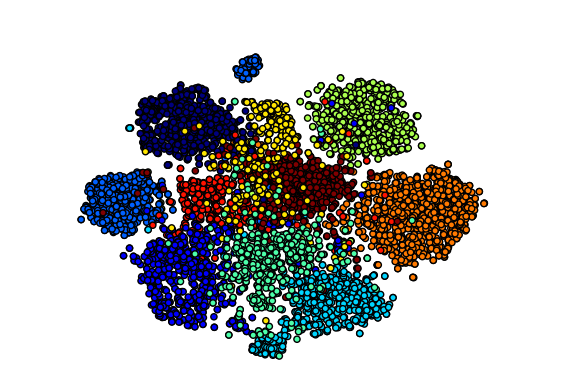
\includegraphics[width=0.85\linewidth]{images/awa_clusters}
\caption[نمایش دسته‌های آزمون مجموعه دادگان AwA ]{
نمایش دوبعدی بوسیله \lr{t-SNE} برای ده دسته‌ی آزمون از مجموعه دادگان AwA با ده رنگ متفاوت نشان داده شده است. درستی فرض قابل خوشه‌بندی در تصویر مشخص است، یعنی ویژگی‌های استخراج شده با استفاده از شبکه‌های عمیق توانایی ایجاد تمایز بالا میان دسته‌ها را دارا هستند.
}
\label{fig:awa_clusters}
\end{figure}

در این بخش ما یک تابع مطابقت جدید بر اساس یک خوشه‌بندی انجام‌شده بر روی داده‌های آزمون تعریف می‌کنیم. اگر فضای نمایش تصاویر دارای این خاصیت باشد که دسته‌های مختلف به صورت خوشه‌های مجزا باشند، استفاده از خوشه‌بندی برای دسته‌بندی برای انتساب برچسب از نظر شهودی توجیه‌پذیر است.
با توجه به نمایش غنی بوجود آمده برای تصاویر توسط شبکه‌های عمیق این فرض در بسیاری از موارد برقرار است. برای نمونه، نمایش \lr{t-SNE} نمونه‌های آزمون مجموعه داده‌های AwA در تصویر
\ref{fig:awa_clusters}
نشان داده شده است و برقراری فرض قابل خوشه‌بندی بودن در آن قابل مشاهده است. این ادعا با استفاده از آزمایش در بخش
\ref{exp:cluster}
اثبات خواهد شد. روش‌های پیشنهادی ما در این فصل بر اساس این ساختار و استفاده از وجود چنین خاصیتی در فضای تصاویر است.
\section{معرفی یک تابع مطابقت}\label{copatibility_function}
یک راه استفاده از چنین خاصیتی در فضای تصاویر، معرفی یک تابع مطابقت است که علاوه بر شباهت نگاشت‌یافته‌ی نمونه‌ها و توصیف‌ها به سایر نمونه‌های در همسایگی هر نمونه نیز وابسته باشد. بدین منظور ما یک تابع مطابقت جدید پیشنهاد می‌دهیم که در آن برچسب تعلق گرفته به هر نمونه به نمونه‌هایی که با آن‌ها در یک خوشه قرار گرفته است وابسته است. به این منظور ابتدا باید یک خوشه‌بندی روی نمونه‌ها انجام شود سپس با استفاده از یک معیار (که یک نمونه از آن را در بخش \ref{simple_method} معرفی می‌کنیم) میزان شباهت خوشه به توصیف تعیین می‌شود. این در مقابل حالتی است که تابع مطابقت میزان شباهت تک تک نمونه‌ها را توصیف‌ها محاسبه می‌کرد.
 در این حالت هر خوشه باید یک برچسب دریافت کند و برچسب اختصاص یافته به هر خوشه، توسط تمام اعضای آن به ارث برده می‌شود. این تابع مطابقت تا کنون در روش‌های موجود برای یادگیری بدون برد استفاده نشده بوده است. این تابع مطابقت قابل اضافه شدن به روش‌های دیگر نیز می‌باشد. به این صورت که پیش‌بینی‌های انجام شده در آن روش را در نظر گرفته و با استفاده از آن‌ها در هر خوشه رای‌گیری انجام دهیم تا برچسبی که کل خوشه دریافت می‌کند تعیین شود. آزمایشات نشان می‌دهند که  اضافه شدن این تابع مطابقت عمل‌کرد روش‌های پایه را بهبود می‌دهد.
%-----------------------------------------------------------Section -----------
\section{یک خوشه‌بندی نیمه‌نظارتی}\label{clustering_method}
عمل‌کرد تابع مطابقت معرفی شده در بخش قبل وابسته به دقت خوشه‌بندی انجام شده روی داده‌هاست. در واقع دقت خوشه‌بندی انجام شده، حد بالای دقت نهایی روش خواهد بود و این در حالتی رخ می‌دهد که هر خوشه برچسبی را دریافت کند که برچسب صحیح  اکثر اعضای آن است. با توجه به این موضوع وجود یک خوشه‌بندی دقیق برای استفاده از این تابع مطابقت ضروری است. البته در آزمایش‌های انجام شده، با استفاده از  الگوریتم خوشه‌بندی
\lr{k-means} \cite{kmeans}
نیز می‌توان به عمل‌کرد پیشگام دست پیدا کند. اما این الگوریتم در خوشه‌بندی نمونه‌های آزمون استفاده‌ای از برچسب‌هایی که برای نمونه‌های آموزش وجود دارد، نخواهد کرد و این اطلاعات می‌توان باعث بهبود عمل‌کرد خوشه‌بندی شود. از طرفی الگوریتم‌های نیمه‌نظارتی موجود برای خوشه‌بندی نیز بر مسئله یادگیری بدون برد تطابق ندارند. در حالت معمول یادگیری نیمه‌نظارتی \cite{chapel06}، مسئله به این صورت تعریف می‌شود که داده‌های برچسب‌دار و بدون برچسب همگی به یک مجموعه دسته‌ی یکسان تعلق دارند و داده‌های بدون برچسب نیز در نهایت برچسب یکسانی با داده‌های برچسب‌دار دریافت می‌کنند. این در حالی‌ست که در مسئله یادگیری بدون برد، نمونه‌های بدون برچسب در دسته‌های مجزا از نمونه‌های برچسب‌دار قرار می‌گیرند. با توجه به این موضوع، یک روش خوشه‌بندی نیمه‌نظارتی پیشنهاد می‌کنیم که با فرض‌های مسئله یادگیری بدون برد منطبق باشد. در این روش خوشه‌بندی همانند k-means عمل می‌شود با این تفاوت که اگر شماره خوشه نمونه‌های دیده شده  برابر با برچسب صحیح آن‌ها نباشد، جریمه‌ای در نظر گرفته می‌شود. تابع هزینه این روش به این صورت تعریف شده است:
\begin{equation} \label{eq:my_clustering}
\min_{R, \boldsymbol{\mu_1, \ldots, \mu_k }}  \sum_{n,k} r_{nk} \normtwo{\mathbf{x_n} - \boldsymbol{\mu_k}} +
 \beta \sum_{n=1}^{N_s} \mathds{1}(\mathbf{r_n} \neq \mathbf{y_n}),
\end{equation}
در این معادله $ \boldsymbol{\mu_1, \ldots, \mu_k }$ مراکز خوشه‌ها و $R$ ماتریس اختصاص خوشه‌هاست، جمله اول همان جمله موجود در تابع هزینه‌ی
\lr{k-means}
است. علاوه بر این، در جمله‌ی دوم برای هر نمونه‌ی برچسب‌دار، اگر به خوشه‌ای تعلق بگیرد که شماره آن با برچسبش متفاوت باشد، جریمه $\beta$ در نظر گرفته می‌شود. در نتیجه این روش، $n_s$ خوشه ابتدایی را به سمت این سوق می‌دهند که همان $n_s$ دسته‌ی دیده شده باشند.  $\beta$ یک فراپارامتر مدل است که اهمیت این جمله اضافه شده را تعیین می‌کند.


% فرض کنید که نمونه‌های $X_u$ با یک روش خوشه‌بندی به $n_u$ خوشه تقسیم شده‌اند و $R$ ماتریس اختصاص خوشه‌ها با نمایش یکی‌یک است.
\section{روش ساده برای دسته‌بندی} \label{simple_method}
در این بخش روشی معرفی می‌شود که همراه با خوشه‌بندی بخش قبل یک چهارچوب برای دسته‌بندی در مسئله یادگیری بدون برد را تشکیل می‌دهند. برای نسبت دادن برچسب به خوشه‌ها، به دنبال یافتن نمایشی از امضای هر دسته در فضای تصاویر به عنوان نماینده آن دسته در فضای تصاویر هستیم. از نظر شهودی مطلوب است که این نماینده‌ها بر مرکز خوشه‌هایی که در فضای تصاویر تشکیل می‌شود منطبق باشند. برای محقق شدن این خاصیت، نگاشت را به صورتی یاد می‌گیریم که در میانگین نمونه‌های دسته‌های آموزش باشد:
\begin{equation} \label{eq:d_definition}
  D = \argmin_D \normf{X_s - D Z_s}^2 + \gamma \normf{D}^2,
\end{equation}
در این معادله، ستون‌های
 $Z_s \in \mathbb{R}^{a \times N_s}$
  امضای دسته‌های نمونه‌های $X_s$ هستند و $\gamma$ یک فراپارامتر است که با اعتبار سنجی تعیین خواهد شد. مسئله تعریف شده برای یافتن نگاشت $D$، امضای کلاس را طوری می‌نگارد که نزدیک به مرکز نمونه‌های آن دسته باشد و این در حالت ایده‌آل همان مرکز خوشه‌ها خواهد بود. در نتیجه این نگاشت برای تعیین دسته‌ها به صورت نزدیک‌ترین همسایه مطلوب بنظر می‌رسد. مسئله بهینه‌سازی
  \eqref{eq:d_definition}
  دارای جواب فرم بسته‌ی زیر است:
  \begin{equation} \label{eq:d_answer}
  D = X_s Z_s^T (Z_s Z_s^T + \gamma I)^{-1}.
\end{equation}

برای تخصیص برچسب به هر خوشه از این رابطه استفاده می‌کنیم:
\begin{equation}
\label{eq:simple_assignment}
\ell(\boldsymbol{\mu_k}) = \argmin_{u=1,\ldots,n_u} \normf{\boldsymbol{\mu_k} - DC_{s(u)}}^2
\end{equation}
و تمامی عناصر خوشه‌ی $k$م برچسب $\ell(\boldsymbol{\mu_k})$ را دریافت می‌کنند.

در این روش سه فراپارامتر وجود دارد، یک پارامتر $\gamma$ در معادله
\eqref{eq:d_definition}
است و دو پارامتر دیگر که مربوط به خوشه‌بندی نیمه‌نظارتی هستند، یعنی $k$ و $\beta$ در معادله
\eqref{eq:my_clustering}.
در آزمایشات عملی دریافتیم که روش به مقدار پارامتر $\gamma$ حساس است در نتیجه مقدار آن توسط یک روند اعتبارسنجی تعیین خواهد شد، نحوه‌ی اعتبار سنجی به صورت دقیق در بخش
\ref{exp:validation}
بیان خواهد شد. در مقابل، مدل به پارامترهای $k$ و $\beta$ حساس نبود، در نتیجه برای ساده و سریع‌تر شدن روند آموزش مقدار آن‌ها را ثابت در نظر گرفته‌ایم. برای $k$ مقدار
$k = n_s + 2n_u$
در نظر گرفته شده است تا هر کدام از دسته‌های دیده‌نشده بتوانند با دو خوشه نمایش داده شوند و در نتیجه پراکندگی و اختلاف میان نمونه‌های یک دسته پوشش داده شود. مقدار $\beta$ نیز در حالتی که داده‌ها به صورت $\norm{x}_1=1$ نرمال شده‌اند، برابر $1$ در نظر گرفته شده است.
در آزمایشات عملی که در فصل
\ref{chap:experiments}
گزارش می‌شود، مشاهده می‌شود که این روش  عمل‌کرد پیشگام در دقت دسته‌بندی بدون برد را روی سه مجموعه دادگان از چهار مجموعه بهبود می‌بخشد.

\subsection{بهینه‌سازی}\label{simple_opt}
 کمینه‌کردن تابع هزینه معرفی شده در رابطه
\ref{eq:my_clustering}،
با توجه به این که $R$ یک رنگ‌آمیزی روی نقاط است، یک مسئله‌ی \nphard است. در نتیجه ما از یک تقریب
مشابه الگوریتم خوشه‌بندی \lr{k-means} استفاده می‌کنیم که یک بهینه محلی برای این تابع را پیدا می‌کند. به این منظور،  یک روند تناوبی میان بهینه کردن بر اساس $R$ و $\mu_k$ها به کار گرفته می‌شود. برای بروز رسانی $\mu_k$ روی اعضای خوشه $k$ میانگین گرفته می‌شود:
\begin{equation} \label{eq:updata_mu}
 \boldsymbol{\mu_k} = \frac{\sum_{n=1}^{N_s + N_u}  \mathds{1}(r_{nk}=1)\mathbf{x_n}}{\sum_{n=1}^{N_s+N_u}\mathds{1}(r_{nk}=1)}.
\end{equation}
برای بروز رسانی $R$ هر نمونه به خوشه‌ای اختصاص می‌یابد که کمترین فاصله را با مرکز آن دارد:
\begin{equation} \label{eq:updata_R}
R_{(n)} = \mathbf{1_{\argmin_k \normtwo{x_n - \mu_k}}}, \quad n=1,\ldots,N_s+N_u
\end{equation}
برای مقداردهی اولیه به $\mu_k$ برای  خوشه‌های مربوط به دسته‌های دیده شده، میانگین عناصر آن‌ها را قرار می‌دهیم:
\begin{equation} \label{eq:init_mu}
 \boldsymbol{\mu_k^0} = \frac{\sum_{n=1}^{N_s + N_u}  \mathds{1}(Y_{s(n)} = \mathbf{1_k})\cdot \mathbf{x_n}}{\sum_{n=1}^{N_s+N_u}\mathds{1}(Y_{s(n)} = \mathbf{1_k})},
\quad 1 \leq k \leq n_s
\end{equation}
برای سایر خوشه‌ها، یعنی خوشه‌های مربوط به دسته‌های دیده نشده از الگوریتم
\lr{k-means++ } \cite{kmeanspp}
استفاده می‌کنیم.
روند کامل این روش دسته‌بندی در الگورتیم
\ref{alg:simple}
بیان شده است.

\شروع{program}
	\begin{enumerate}[label={\arabic*},itemsep=.1em, parsep=.1em]
\فقره {\bf ورودی:} تصاویر و توصیف‌های آموزش و آزمون و برچسب‌های نمونه‌های آموزش $X_s, X_u, Y_s, Z_s, C_u$
\فقره {\bf خروجی:} برچسب‌های پیش‌بینی شده برای نمونه‌های آزمون:$Y_u$
\فقره   $k \in \{ 1,2, \ldots, n_s + n_u \}$
\فقره  $n \in \{ 1,2, \ldots, N_s + N_u \}$
\فقره  $\boldsymbol{\mu_k}$ را برای  $k=1,\ldots,n_s$،  با رابطه \eqref{eq:init_mu} مقداردهی کن.
\فقره  $\boldsymbol{\mu_k}$ را برای $k=n_s+1,\ldots,n_s+n_u$، با استفاده از \lr{k-means++} مقداردهی کن.
\فقره تا همگرایی به یک بهینه‌ی محلی، موارد زیر را تکرار کن

\فقره
 $\qquad$   $ a_n \leftarrow  {\argmin_i \lVert x_n - \mu_i \rVert_2}$ //تخصیص خوشه‌ها
\فقره
 $\qquad$ $\mathbf{\mu_k} \leftarrow \sum_{n} \mathbf{x_n} \mathds{1}(a_n = k) / \sum_n (\mathds{1}(a_n = k) $

\فقره  $  D \leftarrow X_s Y_s^T (Y_s Y_s^T + \gamma I)^{-1}$
\فقره  $l[k] \leftarrow \argmin_j \lVert \mathbf{\mu_k} - (DS_u)_{(j)} \rVert_2$
\فقره   $\mathbf{(Y_u)_{(n)}} \leftarrow \mathbf{1}_{l[a_n]}$
\فقره $Y_u$ را برگردان
\end{enumerate}
\caption{الگوریتم ساده خوشه‌بندی و دسته‌بندی با تابع مطابقت پیشنهاد شده}
\label{alg:simple}
\پایان{program}


%-------------------------------------------------- section
\section{خوشه‌بندی و نگاشت توام} \label{jeac}
روش ارائه شده در فصل قبل، هر چند که به دقت دسته‌بندی بالاتری از روش‌های پیشین دست پیدا می‌کند اما دقت دسته‌بندی در آن توسط دقت خوشه‌بندی صورت گرفته محدود شده است. برای حل این معضل در این روش یک چهارچوب معرفی می‌کنیم که خوشه‌بندی و نگاشت توصیف دسته‌ها به فضای تصاویر در آن به صورت توام انجام شود.
برای این منظور تابع هزینه‌ی زیر پیشنهاد می‌شود:
\begin{align}
\label{eq:joint}
 \min_{R,D} \normf{X_s - D Z_s}^2  &+ \lambda \normf{X_u - D C_u R^T }^2 + \gamma \normf{D}^2 \\
   s.t. \quad & R \in \{0,1\}^{N_u \times n_u}. \nonumber
\end{align}
در این معادله $\gamma$ و $\lambda$ فراپارامترهای مدل هستند. جمله اول و سوم در معاله بالا مشابه رابطه \eqref{eq:d_definition} هستند و تاثیر آن‌ها همانند حالت قبل این است که نگاشت $D$ بتواند امضای دسته‌های دیده نشده را به مرکز تصاویر هر دسته بنگارد. جمله دوم که در این معادله اضافه شده، ذاتا یک جمله خوشه‌بندی است. اگر عبارت بالا را از فرم ماتریسی خارج کرده و بر حسب عناصر $R$ بیان کنیم این مسئله واضح‌تر  خواهد شد:
\begin{equation}
\label{eq:essentialy_clustering}
\sum_{n=N_s+1}^{N_s + N_u} \sum_{k=1}^{n_u} r_{nk} \normtwo{\mathbf{x_n} - D \mathbf{c_k}},
\end{equation}
که مشابه تابع هزینه‌ی
\lr{k-means}
است، با این تفاوت که مراکز خوشه‌ها کاملا آزاد نیستند بلکه مراکز خوشه‌ها باید تصویر امضای دسته‌های دیده نشده باشد که توسط نگاشت $D$ به فضای تصاویر نگاشته شده است. در این حالت برچسب‌های پیش‌بینی شده برای نمونه‌ها همان انتساب‌های آن‌ها به خوشه‌هاست که در طول جریان آموزش توامان با نگاشت $D$ یادگرفته می‌شود. در نتیجه مشکل بیان شده برای روش قبل، در این چهاچوب وجود ندارد. جمله خوشه‌بندی را در این چهارچوب می‌توان به این صورت نیز تعبیر کرد که این جمله یادگیری نگاشت $D$ را به صورتی بهبود می‌دهد که با مشکل جابجایی دامنه در آن وجود نداشته باشد. در حالت عادی یادگیری نگاشت $D$ توسط رابطه
\eqref{eq:d_definition}
تنها از نمونه‌های آموزش برای یافتن $D$ استفاده می‌شد، در نتیجه مشکل جابجایی دامنه برای داده‌های آزمون بوجود خواهد آمد، چرا که این داده‌ها در تعیین نگاشت $D$ بی‌تاثیر بوده‌اند. اما جمله اضافه شده در چهارچوب فوق الزام می‌کند که امضای هر دسته‌ی دیده نشده نزدیک به تعدادی از داده‌های آزمون (که توسط $R$ مشخص می‌شوند) نگاشته شود. این مسئله می‌تواند مانع از مشکل جابجایی دامنه شود. این موضوع در بخش
\ref{exp:discussion}
بیشتر بررسی خواهد شد.
\subsection{بهینه‌سازی}

\شروع{program}[t!]
	\begin{enumerate}[label={\arabic*},itemsep=.1em, parsep=.1em]
\فقره {\bf ورودی:} تصاویر و توصیف‌های آموزش و آزمون و برچسب‌های نمونه‌های آموزش $X_s, X_u, Y_s, Z_s, C_u$
\فقره {\bf خروجی:} برچسب‌های پیش‌بینی شده برای نمونه‌های آزمون:$R$
\فقره $R$ را با خروجی الگوریتم \ref{alg:simple} مقدار دهی کن.
\فقره تا هنگامی که مقدار $R$ تغییر نکند،  تکرار کن:
\فقره $\qquad$  $D$ را با رابطه \eqref{eq:joint_d_update} بروزرسانی کن.
\فقره $\qquad$ عناصر $R$ را با استفاده از رابطه \eqref{eq:joint_r_update} بروزرسانی کن.
\فقره $R$ را برگردان
\end{enumerate}
\caption{الگوریتم یادگیری نگاشت و خوشه‌بندی به صورت توام}
\label{alg:jeac}
\پایان{program}

مسئله بهینه‌سازی رابطه \eqref{eq:joint} بر حسب هر دو متغیر $R$ و $D$ کانوکس نیست اما بر حسب هر کدام از آن‌ها به تنهایی، کانوکس است. در نتیجه برای یافتن یک بهینه محلی از یک روند تناوبی میان بهینه‌کردن بر حسب $R$ و $D$ استفاده می‌کنیم.
برای بروز رسانی $D$ جواب به فرم بسته وجود دارد:
\begin{equation} \label{eq:joint_d_update}
  D = (X_s Z_s^T + \beta X_u R C_u^T) (Z_s Z_s^T + \beta C_u R^T R C_u^T  + \gamma I)^{-1},
\end{equation}
و مقدار بهینه برای $R$، زمانی که $D$ ثابت باشد، با نسبت دادن هر نمونه به نزدیک‌ترین مرکز خوشه به دست می‌آید:
\begin{equation} \label{eq:joint_r_update}
  r_{ij} = \mathds{1}[j = \argmin_{k} \lVert X_{u(i)} - D S_{u(k)} \rVert_2 ].
\end{equation}
در این روند بین بروز رسانی $D$ و $R$ تناوب انجام می‌شود تا جایی که $R$ ثابت بماند یعنی تغییری در برچسب‌های پیش‌بینی شده برای هیچ‌کدام از نمونه‌ها رخ ندهد. در آزمایشات انجام شده این همگرایی همواره در کمتر از ۲۰ بار بروز رسانی به دست می‌آید.
مراحل این روش در الگوریتم \ref{alg:jeac} آمده است.

%--------------------------section
